\documentclass[11pt, a4paper]{report}

\usepackage[utf8]{inputenc}
\usepackage[german, english]{babel} 
\usepackage{amsmath}
\usepackage{amsfonts}
\usepackage{amssymb}
\usepackage{epigraph}

\usepackage{setspace} %linespacing
\onehalfspacing

\usepackage[top=1in, bottom=1in, left=1.25in, right=1in]{geometry} %setting merges

\usepackage[T1]{fontenc}
\usepackage{graphicx}
\usepackage{lmodern}
\usepackage{caption}
\usepackage{siunitx}
\usepackage{tabularx}
\usepackage{listings}
\usepackage{hyphenat}
\usepackage{pdfpages} %including pdfs
\usepackage{chemfig} % drawing chemical figures
\usepackage{gensymb} % \degree symbol
\usepackage{float} %placing floats(H)

\graphicspath{{/home/thiele/Documents/Physik/HiWi/WW/Plots/}}

\begin{document}
\begin{figure}[h]
  \centering
  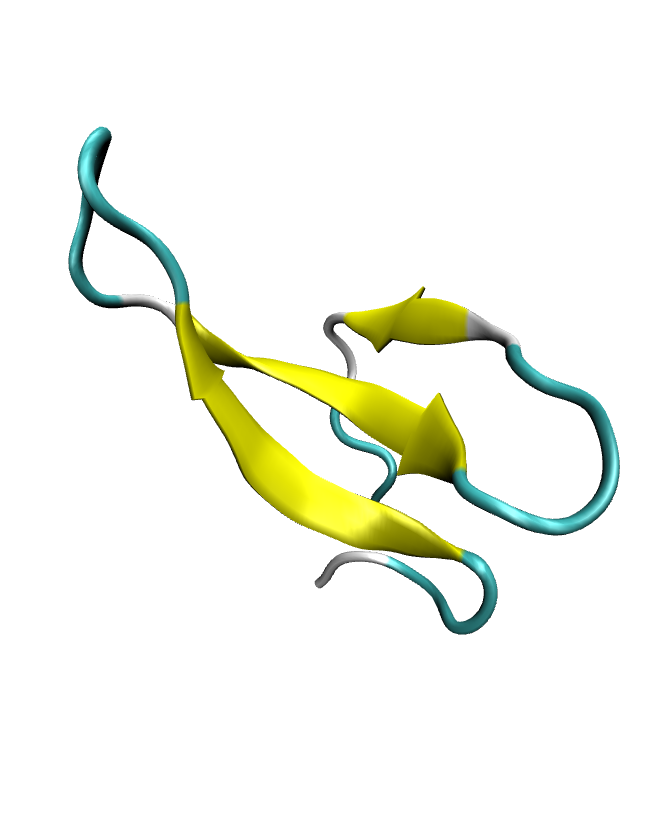
\includegraphics[width=0.8\linewidth]{WW_snapshot2.png}
  \caption{WW}
  \label{fig:WW_snapshot2}
\end{figure}

\begin{figure}[h]
  \centering
  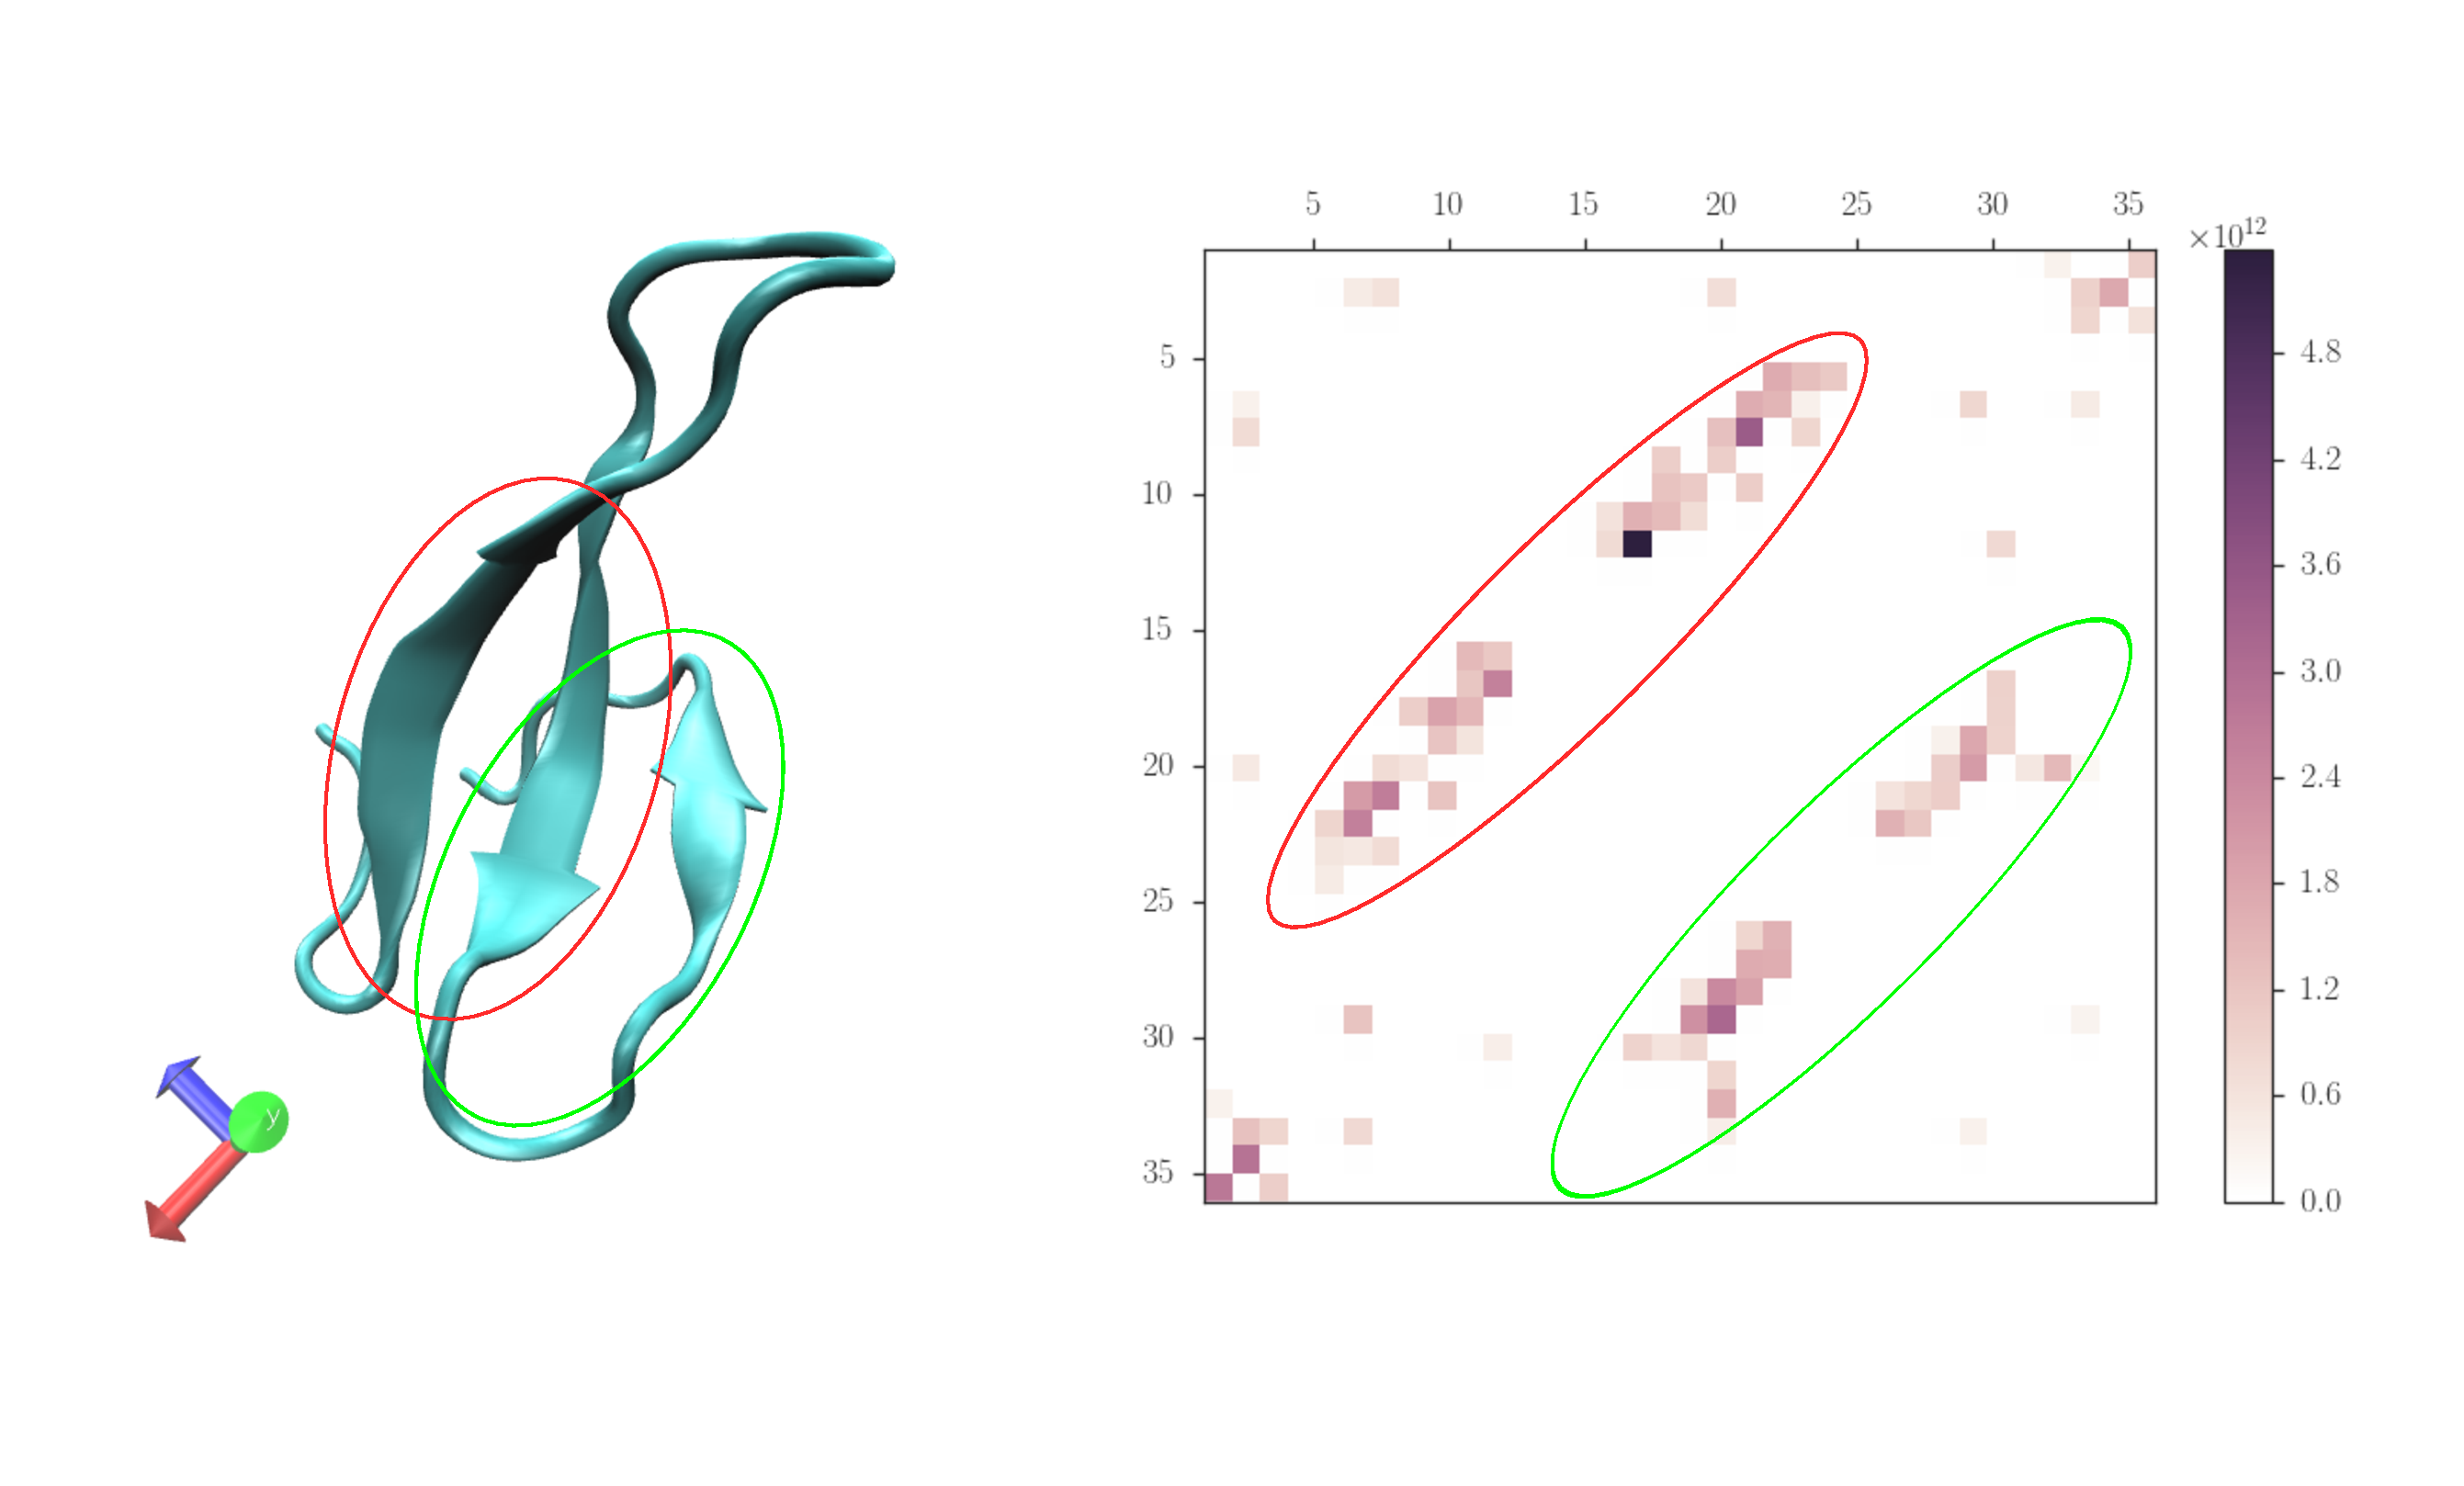
\includegraphics[width=0.8\linewidth]{polar_rates_structure.pdf}
  \caption{Polar contact transition rates between residues.}
  \label{fig:polar_rates_matrix}
\end{figure}

\begin{figure}[h]
  \centering
  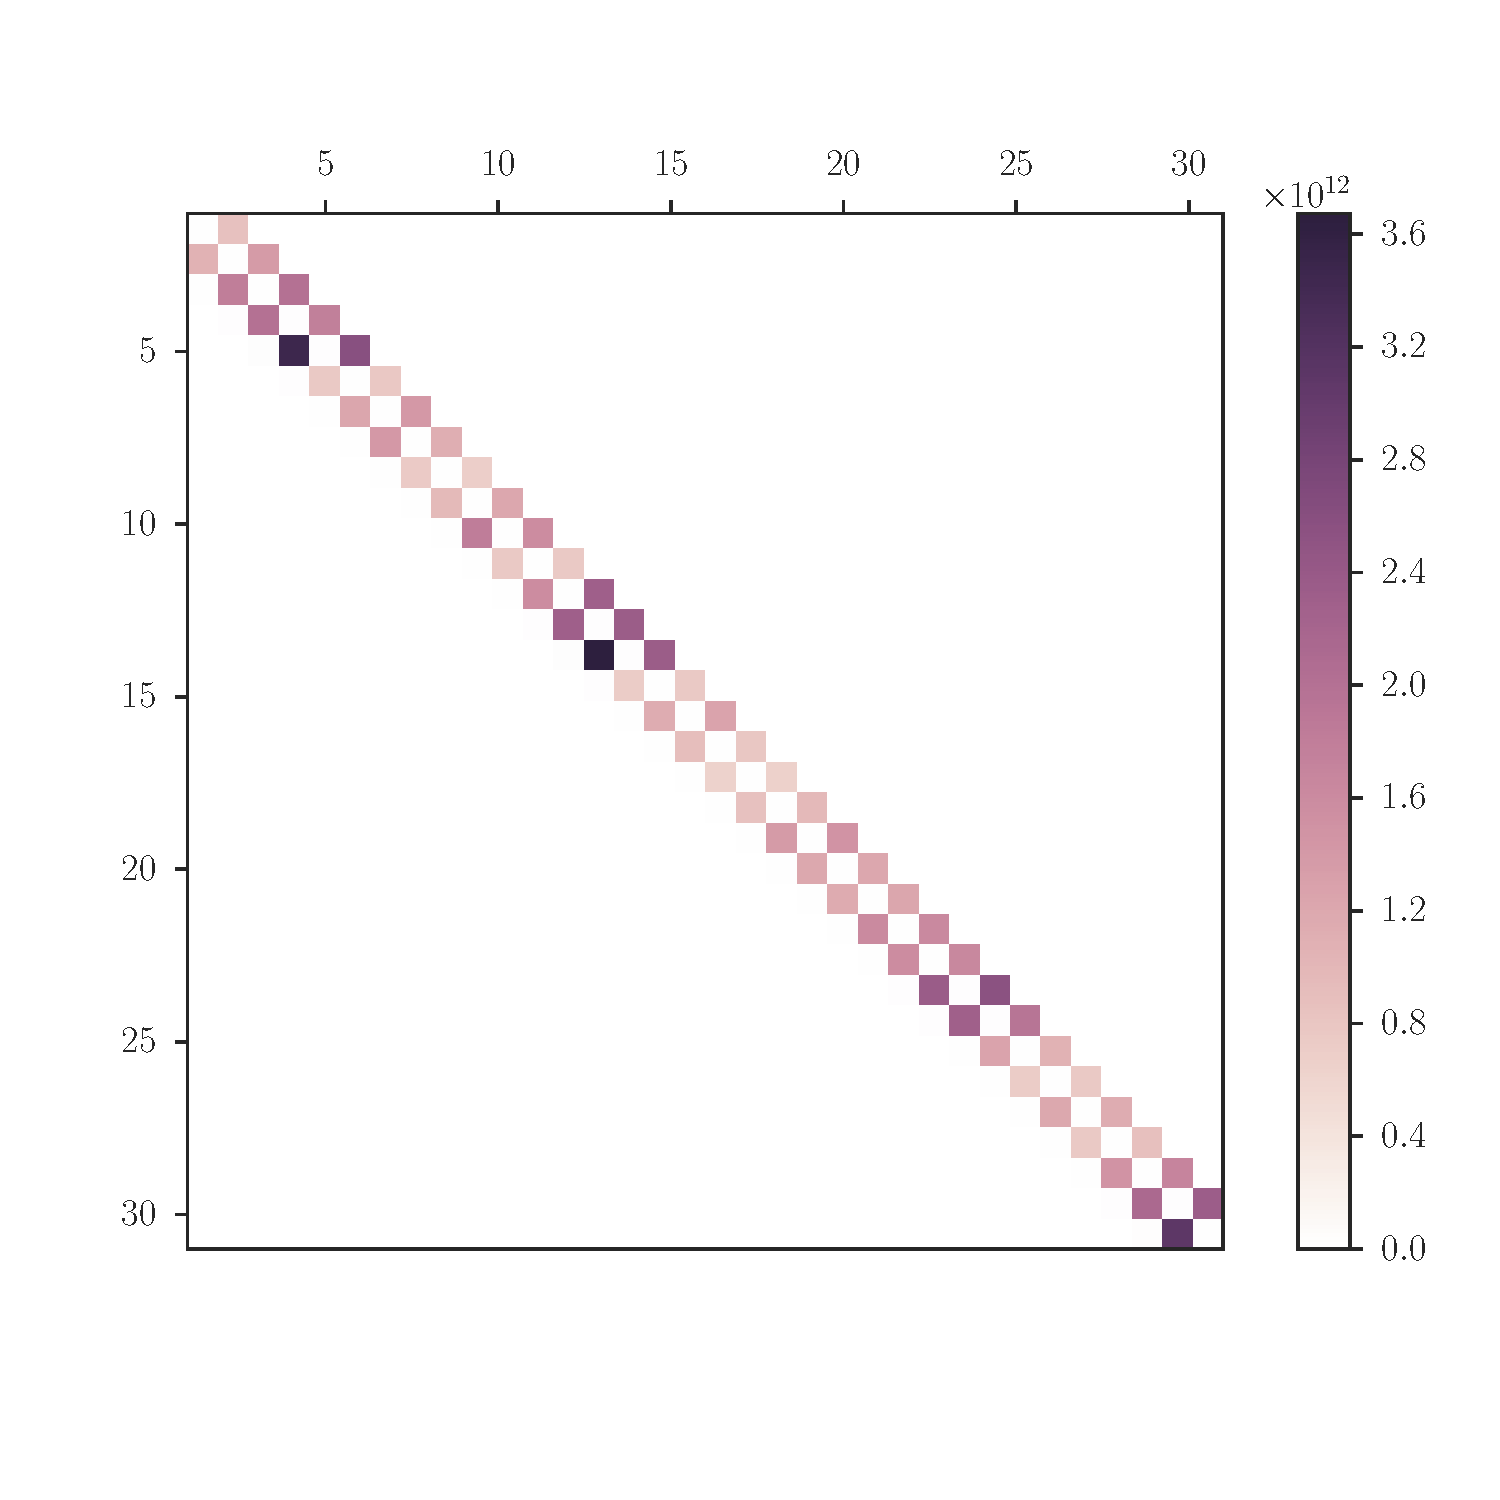
\includegraphics[width=0.8\linewidth]{bonded_rates_matrix.pdf}
  \caption{Backbone transition rates matrix}
  \label{fig:bonded_rates_matrix}
\end{figure}


\section*{MD Data}
\begin{figure}[h]
  \centering
  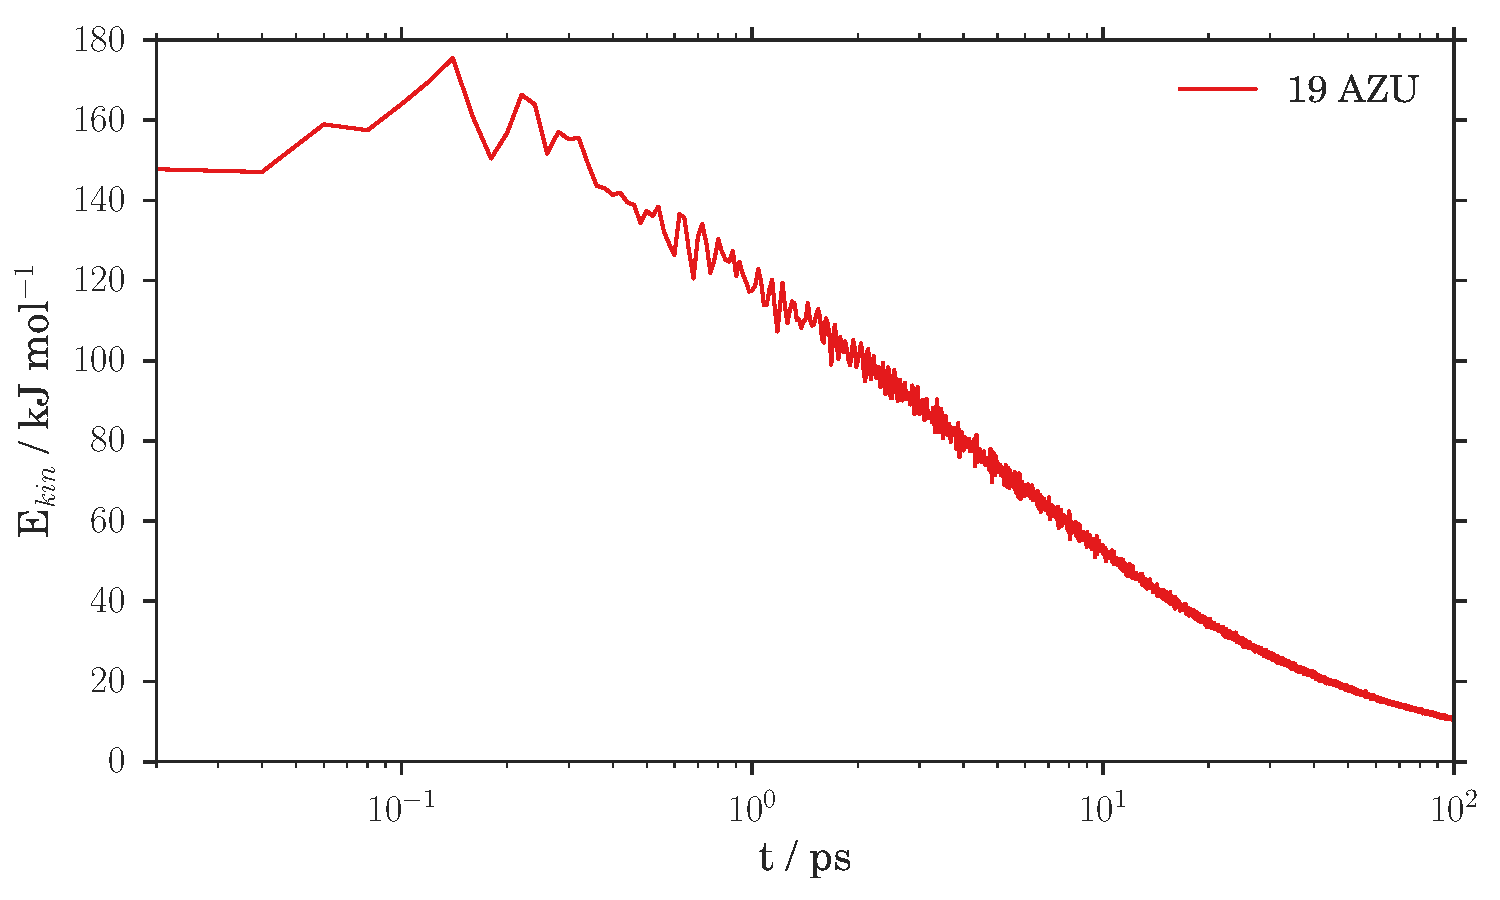
\includegraphics[width=0.8\linewidth]{E_kin_MD_19AZU.pdf}
  \caption{Kinetic energy of the heated residuum AZU 19.}
  \label{fig:E_kin_MD_19}
\end{figure}


\begin{figure}[h]
  \centering
  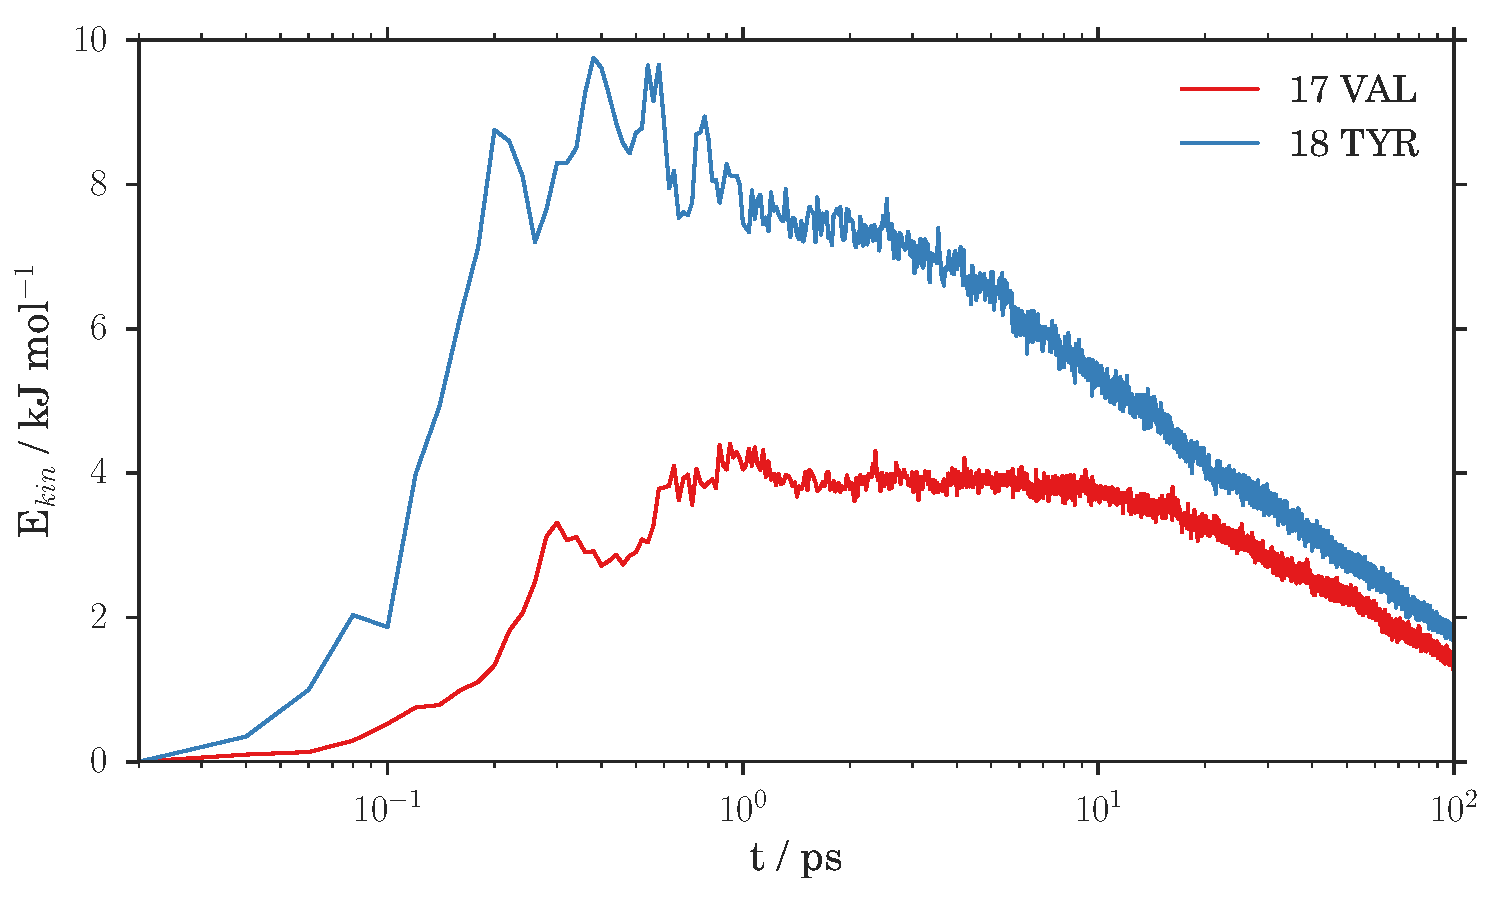
\includegraphics[width=0.8\linewidth]{E_kin_MD_17VAL_18TYR.pdf}
  \caption{Kinetic energy of residues 17 and 18 obtained from MD simulations. Heated residue is AZU 19.}
  \label{fig:E_kin_MD_15_16_17_18}
\end{figure}

\begin{figure}[h]
  \centering
  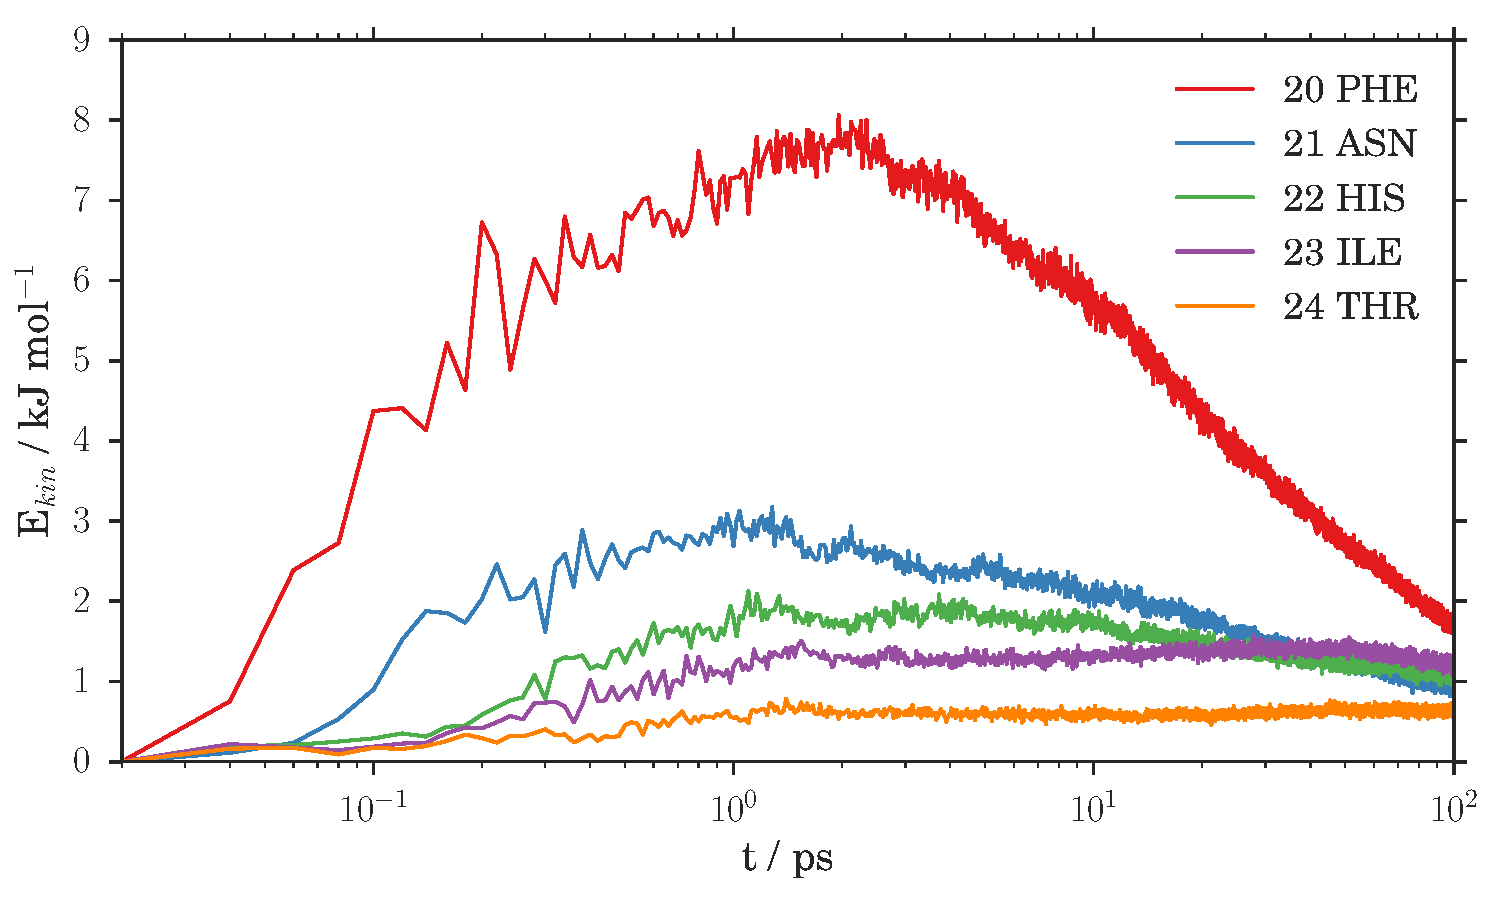
\includegraphics[width=0.8\linewidth]{E_kin_MD_20PHE_21ASN_22HIS_23ILE_24THR.pdf}
  \caption{Kinetic energy of residues 20 to 24 obtained from MD simulations.}
  \label{fig:E_kin_MD_20_21_22_23}
\end{figure}


\begin{figure}[h]
  \centering
  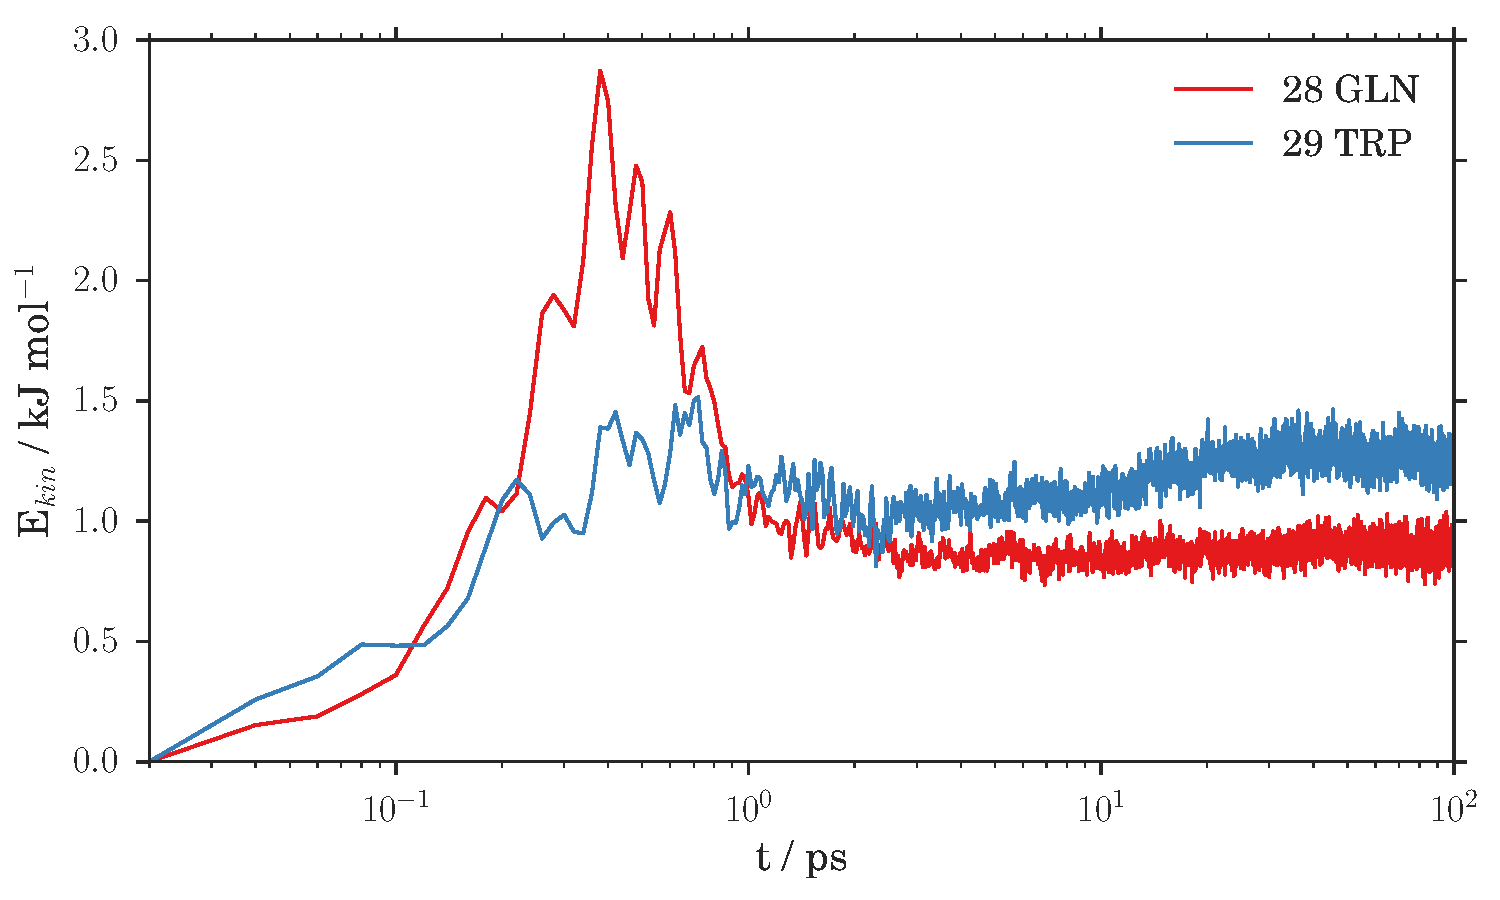
\includegraphics[width=0.8\linewidth]{E_kin_MD_28GLN_29TRP_30GLU_31ARG_32PRO_33SER_34GLY.pdf}
  \caption{Kinetic energy of residues 28 and 29, of which 28 is in polar contact with 19 AZU.}
  \label{fig:E_kin_MD_28GLN_29TRP_30GLU_31ARG_32PRO_33SER_34GLY}
\end{figure}

\begin{figure}[h]
  \centering
  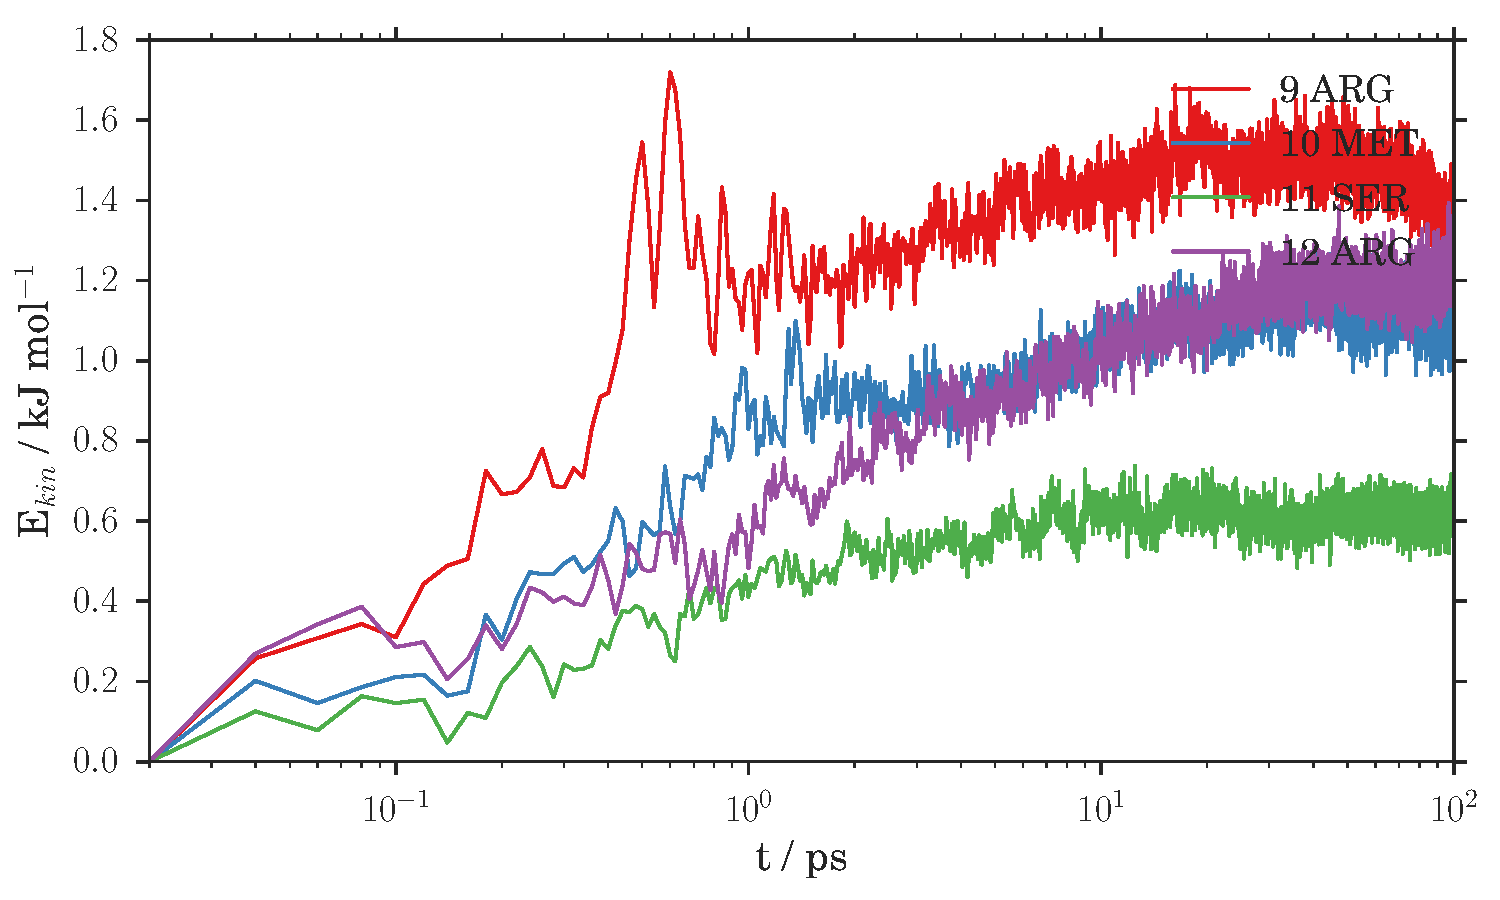
\includegraphics[width=0.8\linewidth]{E_kin_MD_9ARG_10MET_11SER_12ARG.pdf}
  \caption{Kinetic energy of residues 9 to 12 of which 9 ARG is in polar contact with 18 TYR and 20 PHE. }
  \label{fig:E_kin_MEQ_9ARG_10MET_11SER_12ARG}
\end{figure}

\begin{figure}[h]
  \centering
  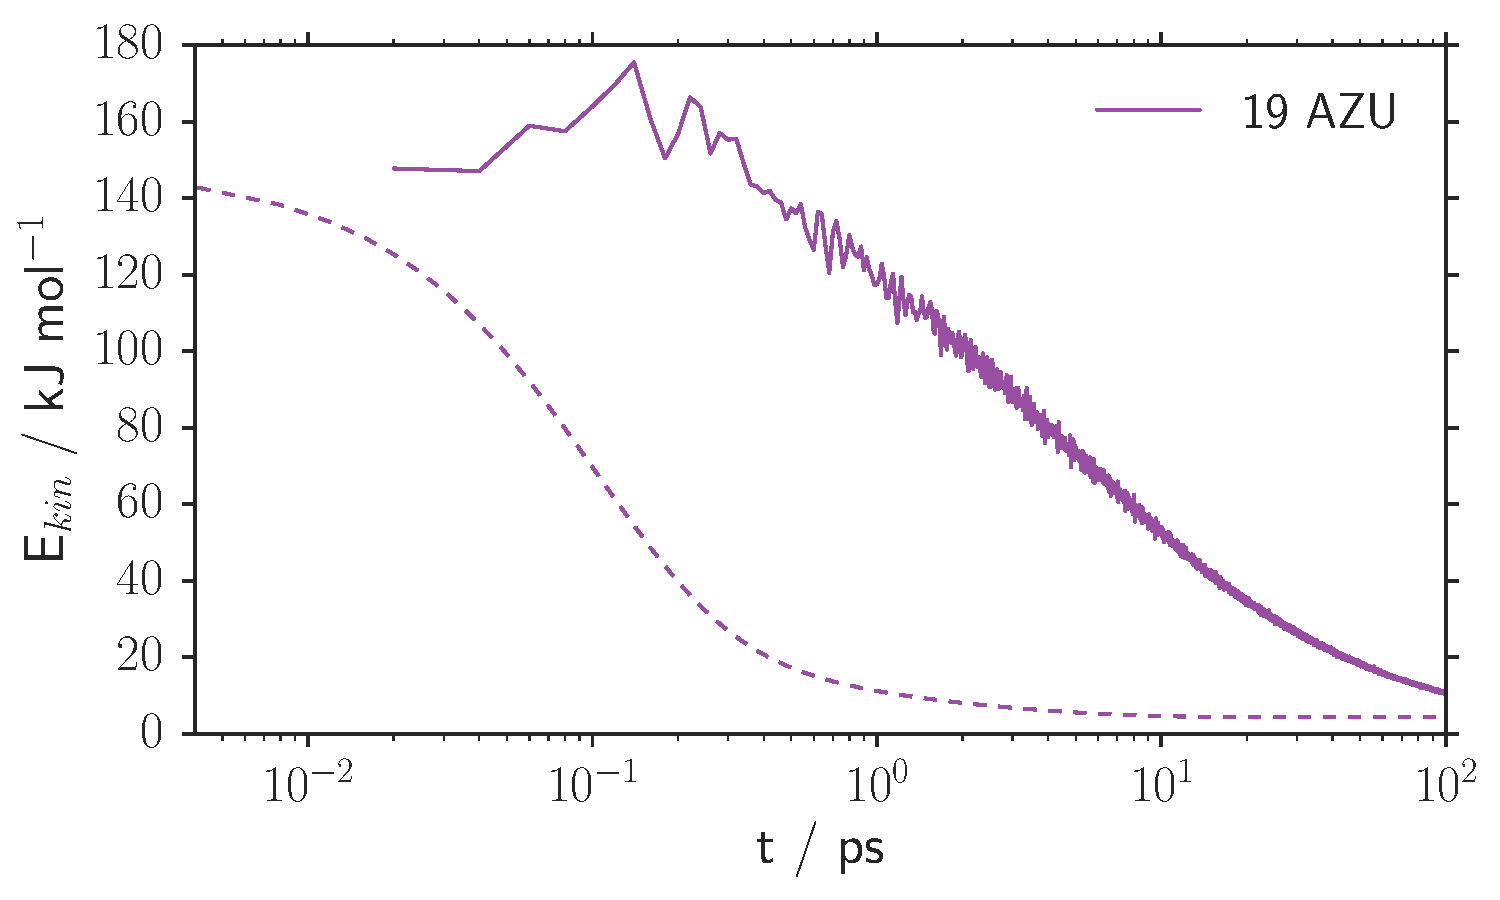
\includegraphics[width=0.8\linewidth]{E_kin_MEQ_MD_19AZU.pdf}
  \caption{Comparison to MEQ simulation for heated residue 19 AZU.}
  \label{fig:E_kin_MEQ_19AZU}
\end{figure}

\begin{figure}[h]
  \centering
  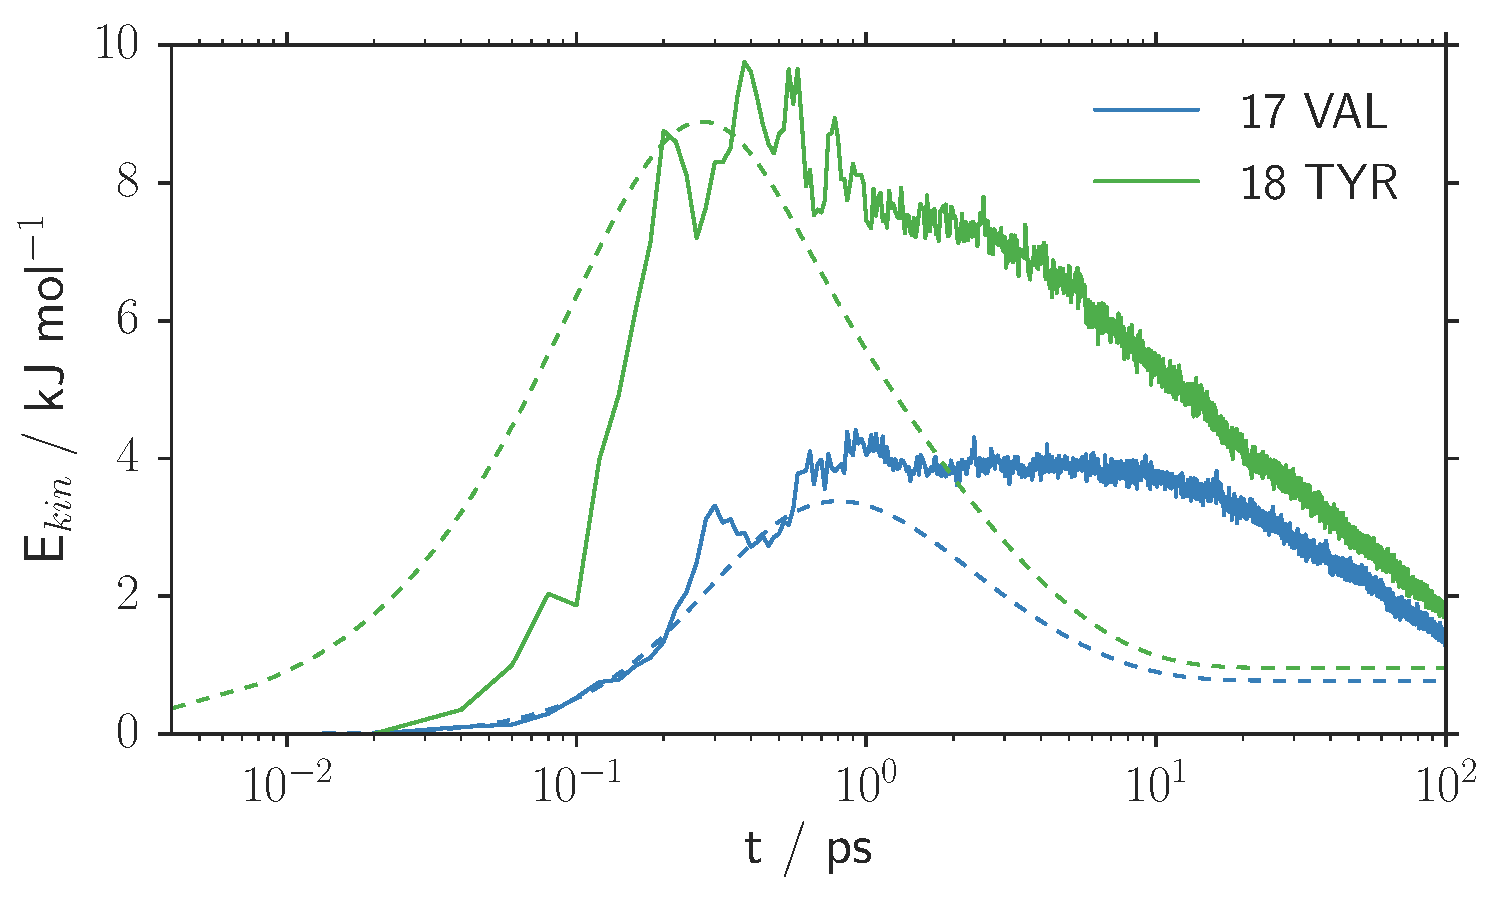
\includegraphics[width=0.8\linewidth]{E_kin_MEQ_MD_17VAL_18TYR.pdf}
  \caption{Comparison to MEQ simulation data for residues 17 and 18.}
  \label{fig:E_kin_MEQ_MD_17VAL_18TYR}
\end{figure}

\begin{figure}[h]
  \centering
  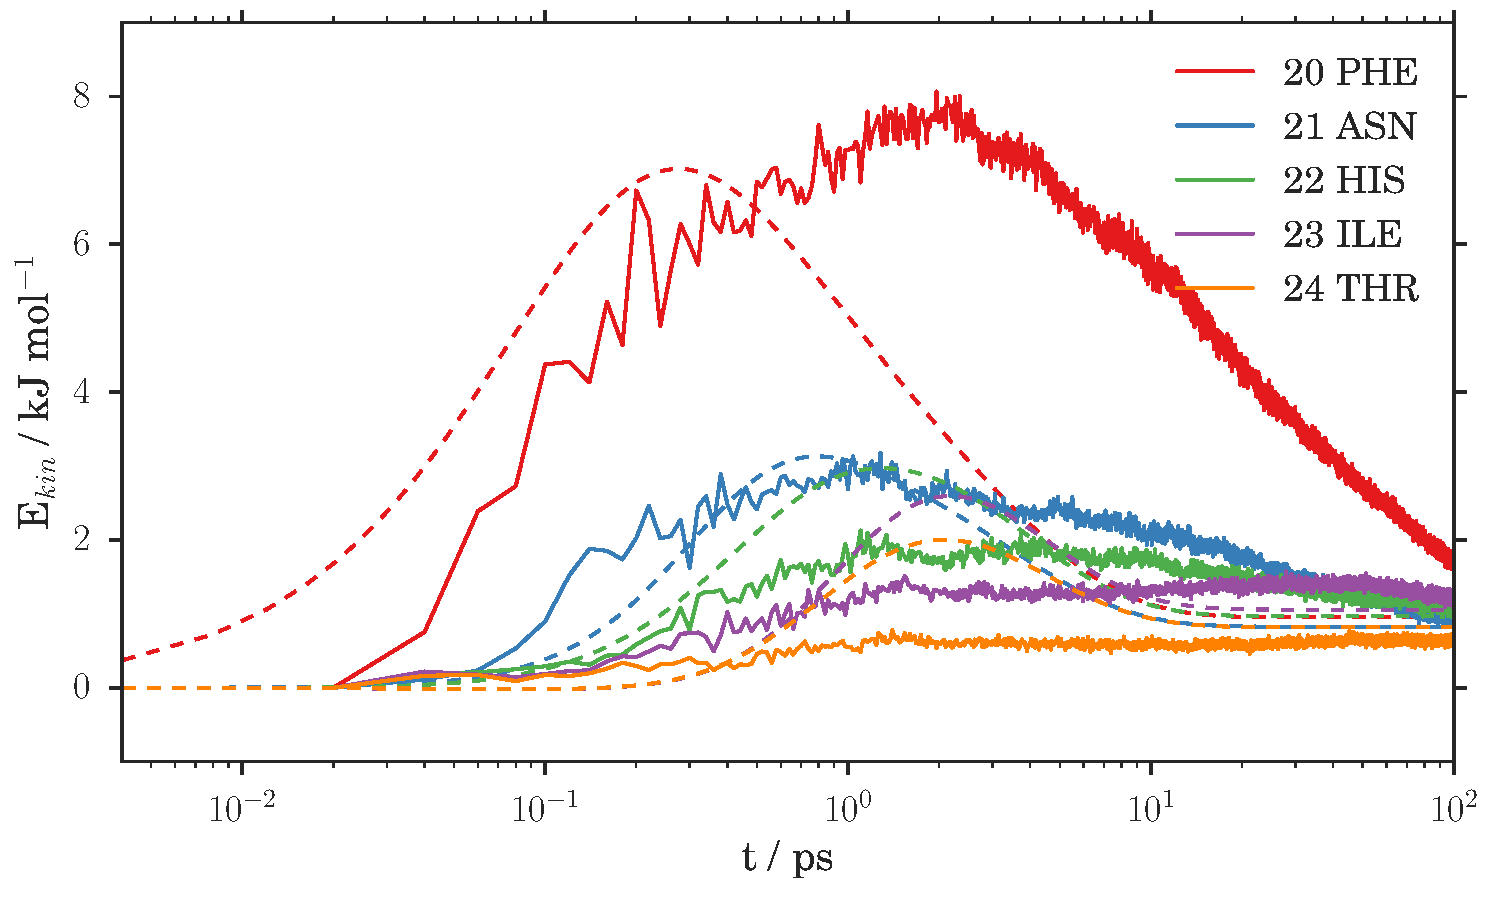
\includegraphics[width=0.8\linewidth]{E_kin_MEQ_MD_20PHE_21ASN_22HIS_23ILE_24THR.pdf}
  \label{fig:E_kin_MEQ_MD_20PHE_21ASN_22HIS_23ILE_24THR}
\end{figure}

\begin{figure}[h]
  \centering
  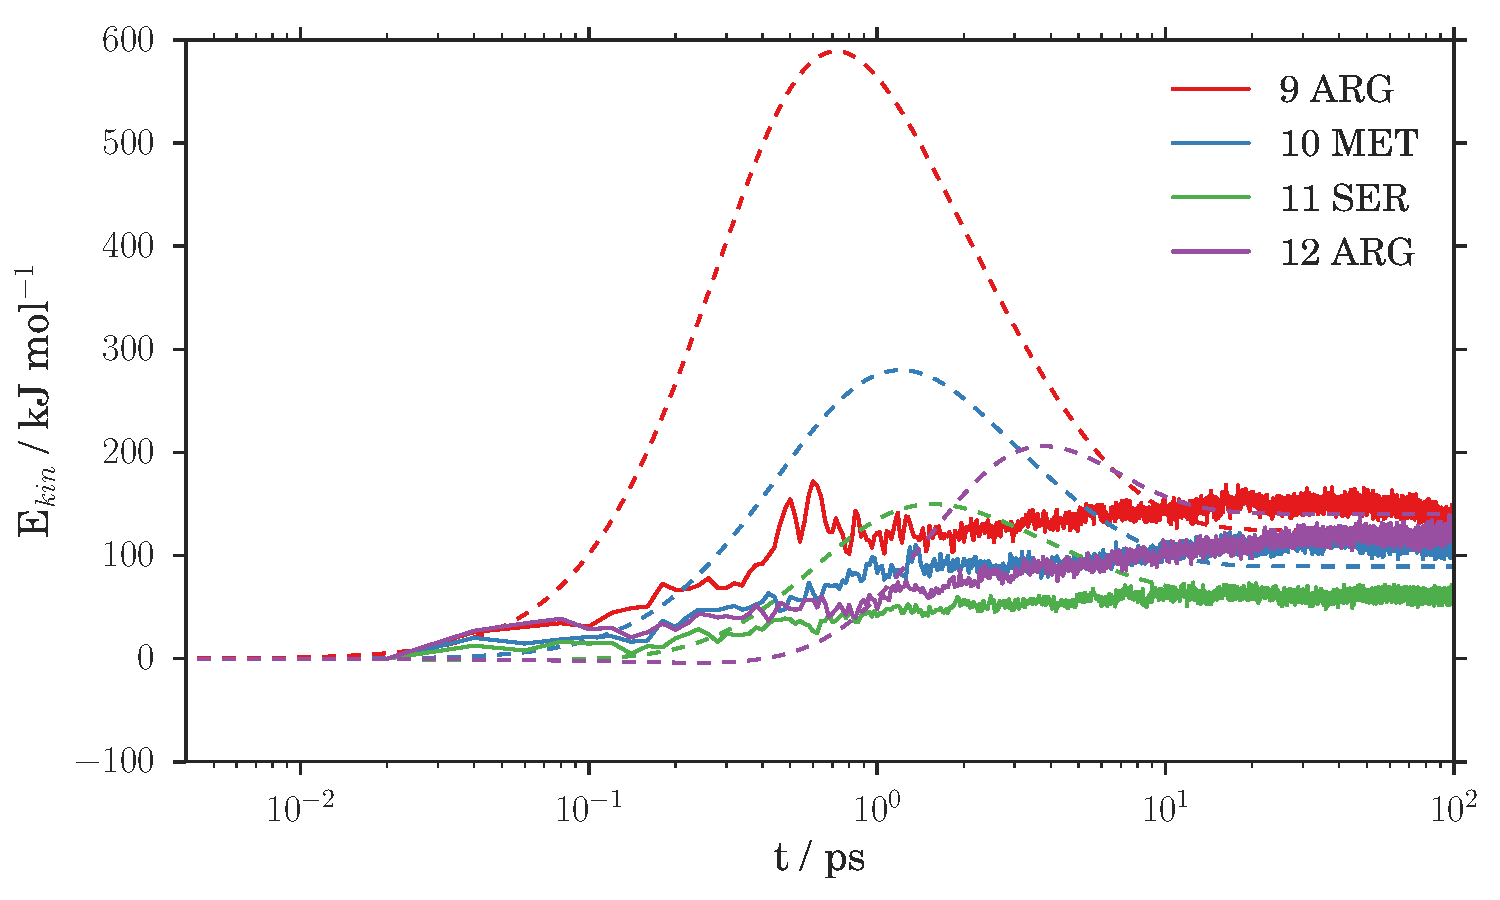
\includegraphics[width=0.8\linewidth]{E_kin_MEQ_MD_9ARG_10MET_11SER_12ARG.pdf}
  \label{fig:E_kin_MEQ_MD_9ARG_10MET_11SER_12ARG}
\end{figure}


\begin{figure}[h]
  \centering
  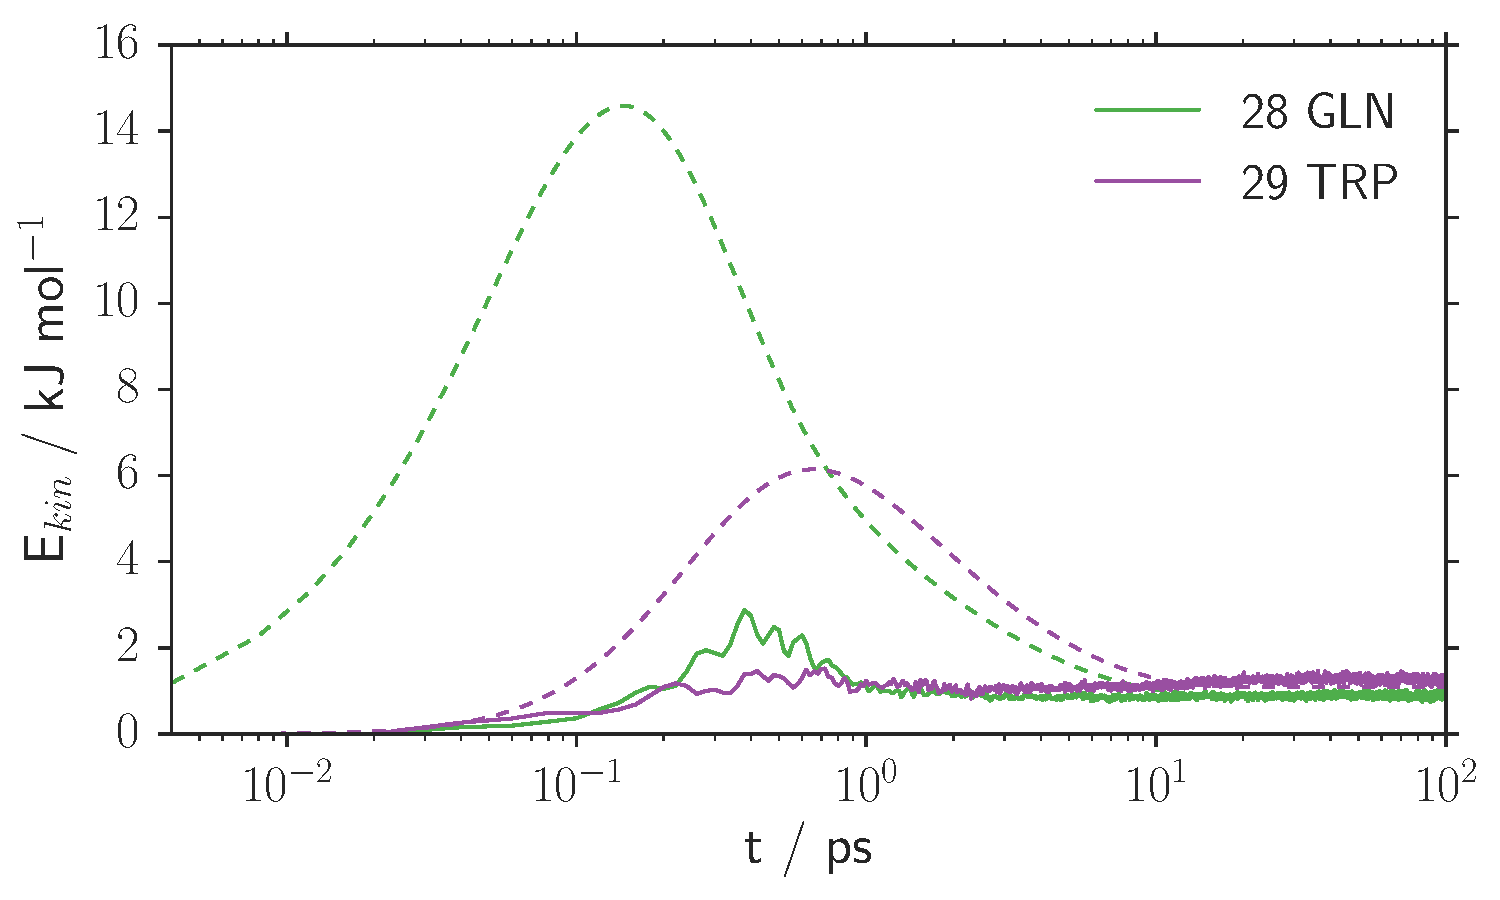
\includegraphics[width=0.8\linewidth]{E_kin_MEQ_MD_28GLN_29TRP_30GLU_31ARG_32PRO_33SER_34GLY.pdf}
  \label{fig:E_kin_MEQ_MD_28GLN_29TRP_30GLU_31ARG_32PRO_33SER_34GLY}
\end{figure}

\end{document}
